\section{Đề xuất giải pháp Kubernetes cho Florus}

\subsection{Mục tiêu chuyển đổi cho hệ thống Florus}

Để khắc phục triệt để các hạn chế về khả năng điều phối và mở rộng của hệ thống cũ, đồ án đề xuất chuyển đổi toàn bộ hạ tầng vận hành sang nền tảng Kubernetes. Đây không chỉ là việc thay đổi công cụ triển khai mà là bước chuyển dịch sang mô hình quản lý tập trung và tự động hóa hoàn toàn, mục tiêu của nhóm trong việc chuyển đổi này gồm:

\begin{itemize}
    \item \textbf{Đảm bảo hoạt động ổn định:} Hệ thống Florus sau quá trình chuyển đổi sang nền tảng Kubernetes cần đảm bảo duy trì tính ổn định trong vận hành, đảm bảo các chức năng, các chỉ số hiệu năng và thời gian uptime đạt mức tương đương hoặc vượt trội so với kiến trúc hiện tại.

    \item \textbf{Cải thiện cơ chế Điều phối và Tự phục hồi:} Thay thế hoàn toàn các script SSH thủ công bằng Kubernetes Controller Manager. Hệ thống sẽ chuyển từ mô hình "Imperative" (dùng các script với các lệnh ssh vào từng node trong hệ thống phân tán để thực hiện hành vi) sang mô hình "Declarative" (chỉ cần khai báo trạng thái cuối cùng của hệ thống, Kubernetes sẽ tự động điều phối để đạt được trạng thái đó). Hơn thế nữa, Kubernetes liên tục giám sát trạng thái thực tế của cụm; nếu một Pod hoặc Node gặp sự cố, hệ thống sẽ tự động khởi tạo lại hoặc di dời ứng dụng sang tài nguyên khả dụng khác mà không cần sự can thiệp của từ bên ngoài.

    \item \textbf{Giải quyết bài toán Service Discovery:} Loại bỏ phương pháp gán cứng địa chỉ IP qua tệp \texttt{/etc/hosts}, đây là cách hard-code và rất kém linh hoạt. Giải pháp mới sử dụng CoreDNS tích hợp sẵn trong Kubernetes kết hợp với đối tượng Service. Các vi dịch vụ sẽ giao tiếp với nhau thông qua DNS Name ổn định. Điều này đảm bảo kết nối giữa các thành phần luôn thông suốt bất kể sự thay đổi về địa chỉ IP hay vị trí vật lý của các Container bên dưới.

    \item \textbf{Đảm bảo tính sẵn sàng cao:} Khắc phục vấn đề "Single Point of Failure" ở tầng ứng dụng bằng cách sử dụng Deployment và ReplicaSet. Mỗi vi dịch vụ quan trọng sẽ được cấu hình chạy đa bản sao. Kubernetes Service sẽ đóng vai trò như một bộ cân bằng tải, phân phối lưu lượng truy cập đều tới các bản sao, đảm bảo dịch vụ hoạt động liên tục ngay cả khi một số instance ngừng hoạt động.

    \item \textbf{Quản lý tài nguyên và Phân chia môi trường:} Sử dụng Namespaces để phân tách logic các môi trường (Dev, Staging, Production) trên cùng một hạ tầng vật lý. Đồng thời, áp dụng cơ chế Resource Quotas và Limit Ranges để giới hạn lượng CPU/RAM tiêu thụ cho từng dịch vụ. Việc này ngăn chặn tình trạng một tiến trình bị lỗi chiếm dụng toàn bộ tài nguyên hệ thống, gây ảnh hưởng dây chuyền đến các dịch vụ khác.

\end{itemize}

\subsection{Yêu cầu trước khi chuyển đổi}

Để hiện thực hóa được việc chuyển đổi hệ thống Florus sang nền tảng Kubernetes, đồ án phải phân biệt được rõ khác biệt căn bản giữa kiến trúc cũ và mới nằm ở triết lý quản lý tài nguyên và trạng thái ứng dụng để có những chuyển đổi mô hình và tư duy phù hợp:

\subsubsection{Từ Mệnh lệnh sang Khai báo} 
\begin{itemize} 
    \item \textbf{Mô hình cũ (Imperative):} Vận hành dựa trên các thao tác can thiệp trực tiếp (\textit{"how"}). Mặc dù đã có các bash script, tuy nhiên bản chất của hệ thống vẫn là người quản trị phải đăng nhập vào từng máy chủ, gõ lệnh khởi chạy container và tự quản lý các tài nguyên. Nếu quy trình sai một bước, hệ thống sẽ lỗi. 
    \item \textbf{Mô hình mới (Declarative):} Vận hành dựa trên định nghĩa trạng thái đích (\textit{"what"}). Nhóm phát triển sẽ cung cấp cho Kubernetes một "bản thiết kế" dưới dạng các file Manifest YAML mô tả trạng thái mong muốn (ví dụ: \textit{"Cần 3 bản sao API Gateway, 2 bản sao Authentication Service,..."}). Kubernetes chịu trách nhiệm tính toán và thực thi các tác vụ cần thiết để đảm bảo hệ thống thực tế luôn khớp với bản thiết kế này mà không cần can thiệp thủ công. 
\end{itemize}

\subsubsection{Từ Quản lý Máy chủ sang Quản lý Tài nguyên} 
\begin{itemize} 
    \item \textbf{Kiến trúc cũ:} Ứng dụng bị gắn chặt với máy chủ vật lý cụ thể. Việc mở rộng đồng nghĩa với việc phải thiết lập thủ công thêm máy chủ mới, gây ra sự phân mảnh. 
    \item \textbf{Kiến trúc mới:} Toàn bộ CPU, RAM và lưu trữ của các máy chủ vật lý được trừu tượng hóa thành một "hồ tài nguyên chung". Kubernetes đóng vai trò như một hệ điều hành của cụm, tự động quyết định đặt ứng dụng vào nơi có tài nguyên rảnh rỗi nhất. Hệ thống không còn phụ thuộc vào bất kỳ máy vật lý đơn lẻ nào.
\end{itemize}

Như vậy, sự chuyển dịch từ tư duy quản lý hành động sang quản lý trạng thái không chỉ đơn thuần là việc thay đổi công cụ, mà là bước chuẩn bị cốt lõi về mặt kiến trúc. Việc thấu hiểu triết lý này là tiền đề bắt buộc để biến hệ thống Florus từ các mảnh ghép rời rạc thành một thực thể thống nhất, có khả năng tự phục hồi và tự động mở rộng, tạo cơ sở vững chắc cho lộ trình hiện thực hóa chi tiết sẽ được trình bày trong phần tiếp theo.

\subsection{Lộ trình hiện thực cụ thể}

Việc chuyển đổi kiến trúc hạ tầng từ Docker Compose sang Kubernetes là một quy trình phức tạp, tiềm ẩn rủi ro về toàn vẹn dữ liệu, độ sẵn sàng cũng như độ tin cậy của hệ thống. Dựa trên các mục tiêu cốt lõi đã xác định, nhóm đề xuất một lộ trình triển khai theo 2 giai đoạn: (1) Thiết lập nền tảng Cluster và (2) Quy trình triển khai ứng dụng:
\newline

\textbf{Giai đoạn 1: Thiết lập nền tảng Cluster} 
\newline
\indent
Quy trình xây dựng "xương sống" cho hệ thống Florus được thực hiện theo trình tự để đảm bảo tính đồng bộ:

\begin{enumerate} 
    \item \textbf{Cài đặt môi trường thực thi:} Cài đặt các thành phần cốt lõi (Containerd, Kubelet, Kubeadm) lên tất cả các máy chủ vật lý. Bước này đồng bộ hóa môi trường, biến các máy tính rời rạc thành các node có khả năng giao tiếp trong cùng một mạng lưới cluster.
    \item \textbf{Thiết lập Control Plane (Master Node):}
    Khởi tạo Node điều khiển trung tâm, nơi chứa các thành phần quản trị cốt lõi như \textit{API Server}, \textit{etcd} (cơ sở dữ liệu lưu trạng thái cluster) và \textit{Scheduler} (bộ lập lịch). Node này đóng vai trò "bộ não", điều phối toàn bộ hoạt động mà không trực tiếp chạy các tác vụ tải nặng.

    \item \textbf{Kết nạp Worker Nodes (Compute Plane):} Các máy chủ còn lại được gia nhập vào cluster với vai trò Worker Node. Đây là nơi thực thi các workload thực tế (Spark Jobs, Backend Services). Tài nguyên của chúng được Control Plane giám sát và cấp phát động.

    \item \textbf{Triển khai lớp mạng:} Thiết lập mạng ảo để đảm bảo các Pods nằm trên các máy vật lý khác nhau có thể giao tiếp trực tiếp qua địa chỉ IP ảo, không cần phải sử dụng File-Besed Service Discovery bằng cách sao chép \texttt{etc/hosts} giữa các máy.
\end{enumerate}

\textbf{Giai đoạn 2: Quy trình triển khai ứng dụng} 
\newline
\indent
Sau khi hạ tầng sẵn sàng, quy trình đưa ứng dụng lên môi trường Production được tự động hóa hoàn toàn:

\begin{enumerate} 
    \item \textbf{Quản lý Artifact tập trung:} Mã nguồn được đóng gói thành các Docker Image và đẩy lên Container Registry. Đây là "nguồn chân lý duy nhất", đảm bảo phiên bản code chạy trên máy Dev và Prod là hoàn toàn giống nhau.

    \item \textbf{Định nghĩa hạ tầng:} Tài nguyên ứng dụng được định nghĩa qua các file YAML, quy định rõ phiên bản Image, giới hạn tài nguyên và chiến lược sao lưu (số lượng bản sao).

    \item \textbf{Cơ chế Lập lịch và Tự phục hồi:} Khi lệnh triển khai được kích hoạt, Kubernetes Scheduler sẽ quét "hồ tài nguyên" để tìm node phù hợp nhất cho ứng dụng. Đặc biệt, cơ chế \textbf{Reconciliation Loop} liên tục giám sát hệ thống: nếu một Worker Node gặp sự cố, Control Plane sẽ tự động phát hiện và di dời các Pod bị ảnh hưởng sang node khác, đảm bảo dịch vụ không bị gián đoạn (Zero Downtime).
\end{enumerate}

Trên cơ sở định hướng chiến lược và lộ trình hai giai đoạn nêu trên, đồ án đã tiến hành các bước hiện thực hóa chi tiết để chuyển đổi hệ thống Florus. Không dừng lại ở mô hình lý thuyết, các phần tiếp theo sẽ trình bày tường minh quá trình kỹ thuật: từ việc thiết lập hạ tầng Cluster thực nghiệm, cho đến chuẩn hóa quy trình triển khai thông qua Helm Charts,... Những nội dung này là minh chứng cụ thể cho tính khả thi và hiệu quả của kiến trúc mới trong việc giải quyết bài toán về vận hành và mở rộng hệ thống.

\subsection{Chiến lược Tái cấu trúc và Chuyển đổi Tài nguyên}

Để hiện thực hóa kiến trúc Kubernetes, đồ án thực hiện quá trình tái cấu trúc toàn diện, chuyển dịch từ cơ chế quản lý dựa trên kịch bản (Script-based) sang cơ chế quản lý dựa trên cấu hình (Configuration-based). Quá trình này bao gồm hai hoạt động song song: Tinh gọn các thành phần lỗi thời và Kiến tạo "nguồn chân lý" mới.

\subsubsection{Tinh gọn "nợ kỹ thuật"} Hệ thống cũ vận hành dựa trên các script mệnh lệnh dày đặc, tạo ra sự phụ thuộc lớn vào cấu trúc vật lý của máy chủ. Để đạt được tính linh hoạt của Cloud-native, nhóm quyết định loại bỏ các thành phần sau khỏi quy trình vận hành Production:

\begin{itemize} 
    \item \textbf{Loại bỏ cơ chế SSH thủ công (cluster.mk):} Tệp tin devops/cluster.mk – trước đây đóng vai trò là "bộ não" điều phối, chứa các vòng lặp logic để SSH vào từng node và thực thi lệnh – sẽ bị loại bỏ hoàn toàn. Trong kiến trúc mới, việc giao tiếp với các node là trách nhiệm của Kubernetes Control Plane thông qua API, không phải của script bên ngoài.

    \item \textbf{Xóa bỏ quản lý DNS tĩnh (`hosts` file):} Việc duy trì tệp devops/cluster/hosts để định danh IP cho các dịch vụ là không còn cần thiết. Kubernetes cung cấp hệ thống CoreDNS tích hợp sẵn, cho phép các dịch vụ gọi nhau thông qua tên định danh mà không cần quan tâm đến địa chỉ IP vật lý.

    \item \textbf{Ngưng sử dụng Docker Compose cho Production:} Các tệp docker-compose-*.yml sẽ ngừng vai trò triển khai trên môi trường thật. Tuy nhiên, nhóm vẫn quyết định lưu trữ chúng như một phương án dự phòng để phục vụ quy trình kiểm thử cục bộ khi không có kết nối tới Cluster.
    
\end{itemize}

\subsubsection{Kiến tạo "Nguồn chân lý" mới} Thay thế cho các kịch bản thủ công là hệ thống các tệp cấu hình Manifest YAML. Đây được coi là "Nguồn chân lý" duy nhất, định nghĩa toàn bộ trạng thái của hệ thống Florus. Dưới đây là bảng tham chiếu chi tiết sự chuyển đổi từ các thành phần Docker Compose sang các đối tượng Kubernetes tương ứng:

\textbf{1. Nhóm quản lý Workload (Stateless \& Stateful):} 

\begin{itemize} 
    \item \textbf{Deployment (thay thế docker compose up):} Đối với các microservice không giữ trạng thái (như API Gateway, Backend), deployment.yaml không chỉ khai báo Image cần chạy mà còn bổ sung các tính năng cao cấp: cơ chế tự phục hồi (Healthcheck), số lượng bản sao (Replicas) và chiến lược cập nhật (Rolling Update). 
    \item \textbf{StatefulSet (thay thế DB Compose Files):} Đối với các dịch vụ cơ sở dữ liệu (MongoDB, PostgreSQL), đồ án sử dụng statefulset.yaml thay vì Deployment. Đối tượng này đảm bảo tính duy nhất và thứ tự khởi chạy, điều kiện tiên quyết để vận hành các cụm cơ sở dữ liệu ổn định. 
\end{itemize}

\textbf{2. Nhóm quản lý Mạng và Định danh (Networking):} \begin{itemize} 
    \item \textbf{Service (thay thế cấu hình mạng thủ công):} Thay vì phải nhớ IP của từng container, service.yaml tạo ra một địa chỉ IP ảo và một tên miền DNS nội bộ ổn định cho từng nhóm Deployment. 
    \item \textbf{Ingress (thay thế Port Binding 5000:5000):} Thay vì mở cổng (expose port) trực tiếp từ container ra máy chủ vật lý – một rủi ro bảo mật, đồ án sử dụng ingress.yaml. Đây là cổng vào duy nhất điều hướng toàn bộ traffic HTTP/HTTPS từ Internet vào các dịch vụ bên trong Cluster. 
\end{itemize}

\textbf{3. Nhóm quản lý Cấu hình và Lưu trữ (Config \& Storage):} 
\begin{itemize} 
    \item \textbf{ConfigMap \& Secret (thay thế .env):} Các biến môi trường được tách khỏi mã nguồn. configmap.yaml lưu trữ thông tin cấu hình thông thường, trong khi secret.yaml mã hóa các thông tin nhạy cảm (như mật khẩu DB, API Key) dưới dạng Base64, tăng cường tính bảo mật so với tệp văn bản thuần .env. 
    \item \textbf{PersistentVolumeClaim - PVC (thay thế Volume Mounts):} Thay vì chỉ định đường dẫn cứng trên máy chủ (ví dụ: ./postgres/data), pvc là một yêu cầu cấp phát tài nguyên trừu tượng. Kubernetes sẽ tự động tìm kiếm và gắn kết (mount) vùng lưu trữ phù hợp, giúp ứng dụng không bị phụ thuộc vào cấu trúc thư mục của một máy chủ cụ thể. 
\end{itemize}

\begin{table}[H]
    \centering
    \small % Giảm cỡ chữ xuống một chút để bảng thoáng hơn
    \caption{Bảng ánh xạ chuyển đổi tài nguyên từ Docker Compose sang Kubernetes Manifests}
    \label{tab:k8s-migration-map}
    % Thiết lập bảng rộng bằng chiều rộng trang (\textwidth)
    % X: Cột tự động co giãn và xuống dòng
    % l: Cột canh trái, độ rộng theo nội dung (dùng cho cột ngắn)
    \begin{tabularx}{\textwidth}{|l|l|X|X|}
    \hline
    \textbf{Tệp Manifest} & \textbf{Phạm vi} & \textbf{Thay thế thành phần cũ} & \textbf{Vai trò và Chức năng} \\ \hline
    
    \texttt{deployment.yaml} & Mỗi Microservice & Lệnh \texttt{docker compose up} đơn lẻ & Khai báo Image, số lượng bản sao, Healthcheck và chiến lược cập nhật ứng dụng không trạng thái. \\ \hline
    
    \texttt{service.yaml} & Mỗi Deployment & Tệp \texttt{hosts} và việc expose cổng thủ công & Tạo địa chỉ IP ảo và tên miền DNS nội bộ ổn định giúp các dịch vụ giao tiếp với nhau. \\ \hline
    
    \texttt{ingress.yaml} & API Gateway & Cấu hình port mapping \texttt{5000:5000} & Đóng vai trò là "Cổng vào" duy nhất, điều hướng traffic HTTP/HTTPS từ bên ngoài vào cụm. \\ \hline
    
    \texttt{configmap.yaml} & Mỗi môi trường & Tệp \texttt{.env} (biến thường) & Lưu trữ các biến cấu hình không nhạy cảm, tách biệt dữ liệu cấu hình khỏi mã nguồn. \\ \hline
    
    \texttt{secret.yaml} & Mỗi môi trường & Tệp \texttt{.env} (biến bí mật) & Mã hóa và lưu trữ an toàn các thông tin nhạy cảm (Password DB, API Key) dưới dạng Base64. \\ \hline
    
    \texttt{statefulset.yaml} & Các Database & Các file compose cho DB (Mongo, Postgres) & Quản lý các ứng dụng có trạng thái, đảm bảo thứ tự khởi chạy và định danh mạng cố định. \\ \hline
    
    \texttt{pvc.yaml} & Các Database & Cấu hình \texttt{volumes} đường dẫn cứng & \textit{PersistentVolumeClaim}: Yêu cầu hệ thống cấp phát vùng lưu trữ bền vững để bảo toàn dữ liệu. \\ \hline
    
    \texttt{Pipeline CI/CD} & Toàn hệ thống & Các script \texttt{Makefile} và \texttt{cluster.mk} & Định nghĩa quy trình tích hợp và triển khai tự động hóa thay thế cho các script thủ công. \\ \hline
    \end{tabularx}
\end{table}


\subsection{Tối ưu hóa quy trình quản lý với mô hình Umbrella Chart}

Mặc dù việc chuyển đổi tài nguyên sang các tệp Manifest YAML (như trình bày tại Bảng \ref{tab:k8s-migration-map}) đã bước đầu hiện thực hóa tư duy Infrastructure as Code, tuy nhiên việc vận hành trực tiếp các tệp tin này vẫn tồn tại những hạn chế đáng kể. Trong thực tế, để khởi chạy toàn bộ hệ thống Florus bằng các file YAML thuần túy, người vận hành phải thực thi hàng loạt câu lệnh \texttt{kubectl apply} theo một trình tự thủ công nghiêm ngặt (ví dụ: phải chạy Database trước, đợi Database khởi động xong mới chạy các Service,...).

\begin{figure}[H]
    \centering
    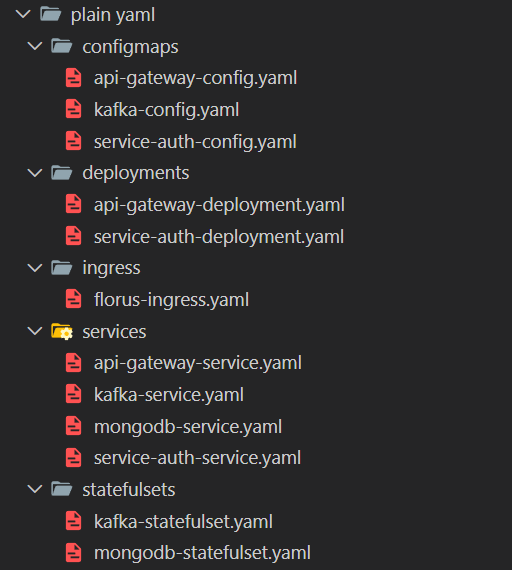
\includegraphics[width=0.6\linewidth]{images/chap 3/plain_yaml.png}
    \vspace{2em}
    \caption{Cấu trúc thư mục các file Manifest truyền thống}
\end{figure}

Cách tiếp cận này dẫn đến tình trạng "bùng nổ cấu hình", khiến quy trình triển khai trở nên rời rạc và dễ gặp lỗi thao tác tương tự như phương pháp thủ công cũ. Để khắc phục triệt để, đồ án nâng cấp quy trình quản lý bằng cách đóng gói toàn bộ các tệp Manifest rời rạc này vào mô hình Helm Umbrella Chart.

\subsubsection{Cơ chế hoạt động}
Thay vì quản lý hàng chục file YAML riêng lẻ, Umbrella Chart hoạt động như một "Chart cha" bao trùm toàn bộ hệ thống. Trong mô hình này: 
\begin{itemize} 
    \item \textbf{Cấu trúc phân tầng:} Các dịch vụ thành phần (Backend, Frontend, Database) được chuyển đổi thành các \textit{Sub-charts} và được khai báo trong tệp \texttt{Chart.yaml} của Umbrella Chart dưới dạng các phần phụ thuộc (\textit{dependencies}). 
    \item \textbf{Triển khai nguyên tử:} Toàn bộ quy trình triển khai phức tạp được tóm gọn lại trong một thao tác duy nhất. Helm sẽ tự động tính toán thứ tự khởi chạy dựa trên đồ thị phụ thuộc, đảm bảo tính đồng bộ của hệ thống. 
\end{itemize}

Việc áp dụng Umbrella Chart đánh dấu bước đệm trong lộ trình chuyển đổi, biến việc triển khai hệ thống phân tán phức tạp trở nên đơn giản và nhất quán như việc cài đặt một phần mềm đơn lẻ.

\begin{figure}[H]
    \centering
    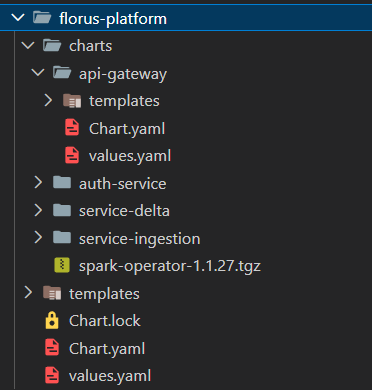
\includegraphics[width=0.6\linewidth]{images/chap 3/umbrella.png}
    \vspace{2em}
    \caption{Cấu trúc thư mục các file Manifest sau khi đã chuyển sang Umbrella Chart}
\end{figure}


\subsubsection{Thách thức kỹ thuật: Giới hạn lưu trữ của Helm Release}

Tuy nhiên, trong quá trình triển khai thực tế mô hình Umbrella Chart nguyên khối chứa toàn bộ các dịch vụ của Florus, nhóm đã gặp phải một rào cản kỹ thuật nghiêm trọng liên quan đến giới hạn của Kubernetes. Cụ thể, khi thực thi lệnh khởi tạo hệ thống:

\begin{lstlisting}[frame=single, basicstyle=\ttfamily\small]
helm upgrade --install florus ./k8s/florus-platform -n florus --create-namespace 
\end{lstlisting}

Hệ thống trả về lỗi gián đoạn quy trình triển khai: 
\begin{quote} 
    \textit{Error: UPGRADE FAILED: create: failed to create: Secret "sh.helm.release.v1.florus.v2" is invalid: data: Too long: may not be more than 1048576 bytes} 
\end{quote}

\textbf{Phân tích nguyên nhân:} Nguyên nhân cốt lõi nằm ở cơ chế quản lý trạng thái của Helm. Theo thiết kế, mỗi bản phát hành của Helm sẽ được lưu trữ dưới dạng một đối tượng \texttt{Secret} (hoặc \texttt{ConfigMap}) trong Kubernetes để phục vụ cho các tính năng lịch sử và rollback. Đối tượng này chứa toàn bộ bản sao của Chart, bao gồm các tệp template đã được render và toàn bộ giá trị cấu hình.

Do hệ thống Florus bao gồm nhiều thành phần phức tạp (Spark, Database, Microservices, Monitoring Stack...), kích thước dữ liệu của bản release đã vượt quá giới hạn cứng \textbf{1MB (1.048.576 bytes)} mà cơ sở dữ liệu \texttt{etcd} của Kubernetes cho phép đối với một đối tượng Secret đơn lẻ\footnote{Kubernetes Documentation, ``Large-Scale Clusters: etcd storage limits,'' 2024. Truy cập: \url{https://kubernetes.io/docs/setup/best-practices/cluster-large/}}.

\subsubsection{Chiến lược phân rã kiến trúc}
Để khắc phục triệt để vấn đề này, đồng thời tăng cường tính linh hoạt trong quản lý vận hành, nhóm quyết định thay đổi chiến lược từ một Umbrella Chart khổng lồ sang mô hình Phân tầng dịch vụ. Hệ thống Florus được tách thành 3 Helm Chart độc lập, quản lý 3 tầng logic riêng biệt:

\begin{itemize} 
    \item \textbf{Tầng 1: Infrastructure Layer (florus-infra):} Chứa các dịch vụ nền tảng có trạng thái và ít thay đổi như Database (MongoDB, PostgreSQL), Object Storage (MinIO) và Message Queue. Việc tách riêng tầng này giúp bảo đảm an toàn dữ liệu, tránh việc cập nhật mã nguồn ứng dụng vô tình làm khởi động lại các database.

    \item \textbf{Tầng 2: Platform Layer (florus-platform):} Chứa các Microservices nghiệp vụ cốt lõi (API Gateway, Auth Service, Backend Services). Đây là tầng có tần suất cập nhật cao nhất, việc tách nhỏ giúp kích thước release luôn nằm trong giới hạn an toàn và quy trình deploy diễn ra nhanh chóng.

    \item \textbf{Tầng 3: Monitoring Layer (florus-monitoring):} Chứa các công cụ giám sát (Prometheus, Grafana). Tầng này hoạt động độc lập, đảm bảo rằng ngay cả khi hệ thống ứng dụng gặp sự cố, hệ thống giám sát vẫn hoạt động để gửi cảnh báo.
\end{itemize}

Việc phân rã này không chỉ giải quyết triệt để lỗi "Secret too long" mà còn tuân thủ nguyên lý Separation of Concerns, giúp quy trình CI/CD có thể tác động độc lập vào từng tầng mà không gây ảnh hưởng chéo đến toàn bộ hệ thống.

\begin{figure}[H]
    \centering
    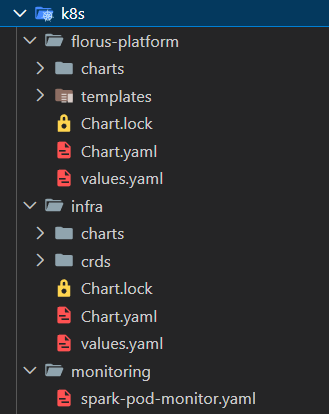
\includegraphics[width=0.6\linewidth]{images/chap 3/umbrella-after.png}
    \vspace{2em}
    \caption{Cấu trúc thư mục các Chart sau khi đã phân lớp}
\end{figure}

\subsubsection{Kỹ thuật tối ưu hóa đặc thù cho Tầng Giám sát}
Trong ba tầng nêu trên, Tầng Giám sát đòi hỏi chiến lược xử lý đặc thù do tính chất cồng kềnh của bộ \textit{kube-prometheus-stack}. Ngay cả khi đã tách riêng, kích thước của các định nghĩa tài nguyên tùy chỉnh (Custom Resource Definitions - CRDs) vẫn đe dọa giới hạn 1MB của Helm Release. Do đó, đồ án áp dụng chiến lược "Tách biệt quản trị":

\begin{itemize}
    \item \textbf{Xử lý CRDs ngoại vi:} Nhóm không để Helm quản lý các CRDs nặng nề này. Thay vào đó, chúng được cài đặt riêng biệt thông qua cơ chế \texttt{Server-Side Apply} của kubectl, sau đó Prometheus được triển khai qua Helm với cờ \texttt{--set crds.enabled=false}. Điều này giảm thiểu đáng kể kích thước của bản Release.
    
    \item \textbf{Cấu hình Service Discovery động:} Thay vì lưu trữ toàn bộ mã nguồn Prometheus, đồ án chỉ duy trì tệp cấu hình cầu nối \texttt{spark-pod-monitor.yaml}.
    \begin{quote}
        \textit{Cơ chế hoạt động:} Prometheus Operator sẽ quét tệp cấu hình này, tự động phát hiện các Spark Driver Pods đang hoạt động và bắt đầu thu thập metrics qua cổng \texttt{spark-ui} mà không cần can thiệp vào mã nguồn lõi của Prometheus.
    \end{quote}
\end{itemize}

\subsection{Thách thức về Bảo toàn Nghiệp vụ Dữ liệu}

Một trong những rào cản lớn nhất trong quá trình chuyển đổi hệ thống Florus không nằm ở các lỗi kỹ thuật bề nổi, mà nằm ở tính chất "Data-Intensive" của hệ thống. Khác với việc di dời các ứng dụng Web (Stateless) thông thường – nơi việc thay đổi môi trường ít ảnh hưởng đến logic – Florus sở hữu các đường ống xử lý dữ liệu phức tạp với sự ràng buộc chặt chẽ giữa tính toán và lưu trữ.

Việc thay thế các thành phần cốt lõi của Platform (như chuyển từ HDFS sang MinIO - sẽ được nói ngay say đây, hay từ Yarn/Docker sang K8s Scheduler) tương đương với việc thay thế "trái tim" của hệ thống đang chạy. Điều này đặt ra một thách thức nghiêm trọng:

\begin{itemize} 

    \item \textbf{Sự nhạy cảm của Nghiệp vụ:} Trong các bài toán xử lý dữ liệu lớn, một sự thay đổi nhỏ ở tầng hạ tầng (như Block size, Network latency, hay cơ chế Consistency) có thể dẫn đến sai lệch hoàn toàn trong kết quả phân tích cuối cùng hoặc làm vỡ cấu trúc dữ liệu.

    \item \textbf{Yêu cầu thấu hiểu hệ thống:}
Quá trình migrate không thể thực hiện theo kiểu "sao chép nguyên trạng" máy móc. Nhóm đồ án buộc phải thấu hiểu tường tận bản chất luồng dữ liệu, cơ chế đọc/ghi của Spark và các phụ thuộc ngầm định trong mã nguồn cũ. Bất kỳ quyết định thay thế công nghệ nào cũng phải được đối chiếu ngược lại với logic nghiệp vụ để đảm bảo tính đúng đắn được bảo toàn tuyệt đối.

\end{itemize}

Chính vì đặc thù này, các quyết định kỹ thuật trong phần tiếp theo (như lựa chọn MinIO hay Spark Operator) không chỉ dựa trên tiêu chí hiệu năng, mà ưu tiên hàng đầu là sự tương thích về hành vi với nghiệp vụ dữ liệu sẵn có.

\subsection{Lựa chọn giải pháp lưu trữ: HDFS hay Object Storage?}
Trong kiến trúc Big Data truyền thống, HDFS (Hadoop Distributed File System) luôn là xương sống lưu trữ mặc định. Tuy nhiên, khi chuyển dịch sang môi trường Cloud-native với Kubernetes, nhóm nghiên cứu đã phải đối mặt với câu hỏi cốt tử: \textit{"Liệu có nên tiếp tục triển khai HDFS trên Kubernetes hay không?"}. Dưới đây là phân tích chi tiết dẫn đến quyết định thay thế HDFS bằng MinIO.

\subsubsection{Xung đột kiến trúc và Vấn đề Data Locality}
HDFS và Kubernetes sinh ra ở hai kỷ nguyên công nghệ khác nhau với những triết lý thiết kế đối lập, tạo nên sự khập khiễng khi tích hợp:

\begin{itemize}
    \item \textbf{HDFS (Kỷ nguyên 2006 - Move Compute to Data):}Trong bối cảnh mạng nội bộ còn chậm và đắt đỏ, HDFS được thiết kế để tối ưu hóa việc đọc/ghi cục bộ. NameNode cần biết chính xác block dữ liệu nằm trên ổ cứng vật lý nào để điều phối MapReduce/Spark chạy ngay tại node đó. Triết lý này dựa chặt vào phần cứng vật lý.
    \item \textbf{Kubernetes (Kỷ nguyên Cloud Native - Disaggregated Storage \& Compute):} Ngược lại, Kubernetes coi các Pod là đối tượng phù du, có thể bị hủy và tái tạo ở bất kỳ node nào. Triết lý hiện đại ưu tiên việc \textbf{tách rời tính toán và lưu trữ}. Dữ liệu không nằm trên ổ cứng của node chạy ứng dụng mà nằm ở các hệ thống lưu trữ qua mạng (Network Storage) được gắn vào qua Persistent Volume.
\end{itemize}

\textbf{Hệ quả:} Khi cưỡng ép chạy HDFS trên Kubernetes, lợi thế lớn nhất là \textbf{Data Locality} bị triệt tiêu hoàn toàn.

\begin{enumerate}
    \item HDFS "lầm tưởng" nó đang ghi xuống ổ đĩa cục bộ, nhưng thực tế nó đang ghi qua mạng xuống hạ tầng lưu trữ Block Storage bên dưới.
    \item Spark chạy trên K8s nghĩ rằng nó đang đọc dữ liệu tại chỗ, nhưng thực tế dữ liệu lại đang nằm ở một node khác.
\end{enumerate}

Điều này dẫn đến "overhead chồng overhead": gánh nặng của lớp ảo hóa mạng K8s cộng với overhead của giao thức HDFS khiến hiệu năng hệ thống thậm chí chậm hơn cả việc dùng S3 native hoặc chạy Bare Metal.

\subsubsection{Thách thức trong vận hành và tích hợp}
Ngoài vấn đề hiệu năng, HDFS còn bộc lộ những hạn chế nghiêm trọng về khả năng bảo trì trong môi trường Container:

\begin{itemize}
    \item \textbf{Cơ chế WebHDFS phức tạp:} Để upload một file, client phải thực hiện chuỗi 3 API liên tiếp (\texttt{MKDIRS} $\rightarrow$ \texttt{CREATE} $\rightarrow$ \texttt{PUT}). Trong môi trường mạng đóng gói của Docker/K8s, việc điều hướng các request này qua Ingress/Service thường xuyên gặp lỗi kết nối hoặc sai lệch port.
    \item \textbf{Gánh nặng quản trị:} Để vận hành HDFS, nhóm phải duy trì một hệ sinh thái cồng kềnh gồm NameNode, DataNode, ZooKeeper và cấu hình Kerberos phức tạp trong các Dockerfile. Điều này đi ngược lại tiêu chí tinh gọn của đồ án.
    \item \textbf{Vấn đề Hardcoded Path:} Các thư viện cũ thường gắn chặt với giao thức \texttt{hdfs://}, gây khó khăn cực lớn khi muốn mở rộng hoặc di chuyển môi trường.
\end{itemize}

\subsubsection{Giải pháp thay thế: MinIO và S3 API}
Để giải quyết các vấn đề trên, đồ án lựa chọn MinIO – một hệ thống lưu trữ đối tượng (Object Storage) hiệu năng cao, tương thích hoàn toàn với chuẩn S3 API. MinIO sinh ra là để dành cho Kubernetes với triết lý phù hợp:

\begin{table}[H]
    \centering
    \renewcommand{\arraystretch}{1.5} % Tăng khoảng cách dòng cho thoáng
    \caption{So sánh kỹ thuật giữa HDFS và MinIO}
    \label{tab:hdfs-vs-minio}
    \begin{tabularx}{\textwidth}{@{}l X X@{}} % @{} để bỏ lề thừa 2 bên
        \toprule
        \textbf{Tiêu chí} & \textbf{HDFS (Legacy)} & \textbf{MinIO (Cloud-native)} \\
        \midrule
        
        \textbf{Triết lý} & Mang tính toán đến dữ liệu (Data Locality) & Tách rời tính toán và lưu trữ (Disaggregated) \\
        
        \textbf{Giao thức} & RPC (nhanh nội bộ), WebHDFS (chậm, phức tạp) & HTTP/REST (S3 API chuẩn công nghiệp) \\
        
        \textbf{Mô hình dữ liệu} & File System phân cấp (có thư mục thật), hỗ trợ Append & Object Storage (Flat namespace), Bất biến (Immutable) \\
        
        \textbf{Quản lý file} & Atomic Rename O(1) & Thư mục là ảo (Prefix). Rename = Copy + Delete \\
        
        \textbf{Khả năng mở rộng} & Mở rộng Storage buộc phải thêm cả CPU/RAM (DataNode) & Mở rộng độc lập Storage và Compute tùy nhu cầu \\
        
        \bottomrule
    \end{tabularx}
\end{table}

\subsubsection{Đánh giá về tính toàn vẹn dữ liệu (Data Compatibility)}
Một lo ngại lớn khi chuyển đổi từ HDFS sang MinIO là tính tương thích của dữ liệu. Tuy nhiên, qua thực nghiệm, nhóm khẳng định vấn đề này hoàn toàn được giải quyết nhờ lớp trừu tượng hóa của Spark:
\begin{itemize}
    \item \textbf{Định dạng tệp là yếu tố quyết định:} Cả HDFS và MinIO thực chất đều chỉ là nơi chứa các chuỗi byte (Blob storage). Việc dữ liệu có đọc được hay không phụ thuộc vào định dạng tệp như Parquet, Avro, CSV chứ không phụ thuộc vào nơi lưu trữ.
    \item \textbf{Vai trò của Spark:} Spark đóng vai trò là "trọng tài" xử lý dữ liệu. Schema được định nghĩa trong code ứng dụng. Dù đọc tệp Parquet từ \texttt{hdfs://} hay \texttt{s3a://}, Spark đều giải mã và tạo ra cùng một DataFrame kết quả. Do đó, việc thay đổi tầng lưu trữ bên dưới hoàn toàn \textbf{an toàn về mặt dữ liệu} và không ảnh hưởng đến logic nghiệp vụ phía trên.
\end{itemize}

Kết luận, việc chuyển dịch sang MinIO không chỉ giúp hệ thống Florus tương thích tốt hơn với Kubernetes mà còn đơn giản hóa đáng kể quy trình vận hành, tuân thủ đúng chuẩn công nghiệp hiện đại.